\section{Introduction}
\label{sec:introduction}

% state the learning objective 
The objective of this laboratory assignment is to study a RC circuit containing a
AC voltage source $V_s$, a capacitor $C$, a voltage controlled current
source $I_b$, a current controlled voltage source $V_d$ and resistors,
$R_1$, $R_2$, $R_3$, $R_4$, $R_5$, $R_6$ and $R_7$. The circuit can be seen in Figure \ref{fig:t2}.

In Section~\ref{sec:analysis}, a theoretical analysis of the circuit is
presented. In Section~\ref{sec:simulation}, the circuit is analysed by
simulation, and the results are compared to the theoretical results obtained in
Section~\ref{sec:analysis}. The conclusions of this study are outlined in
Section~\ref{sec:conclusion}.

\begin{figure}[H] \centering
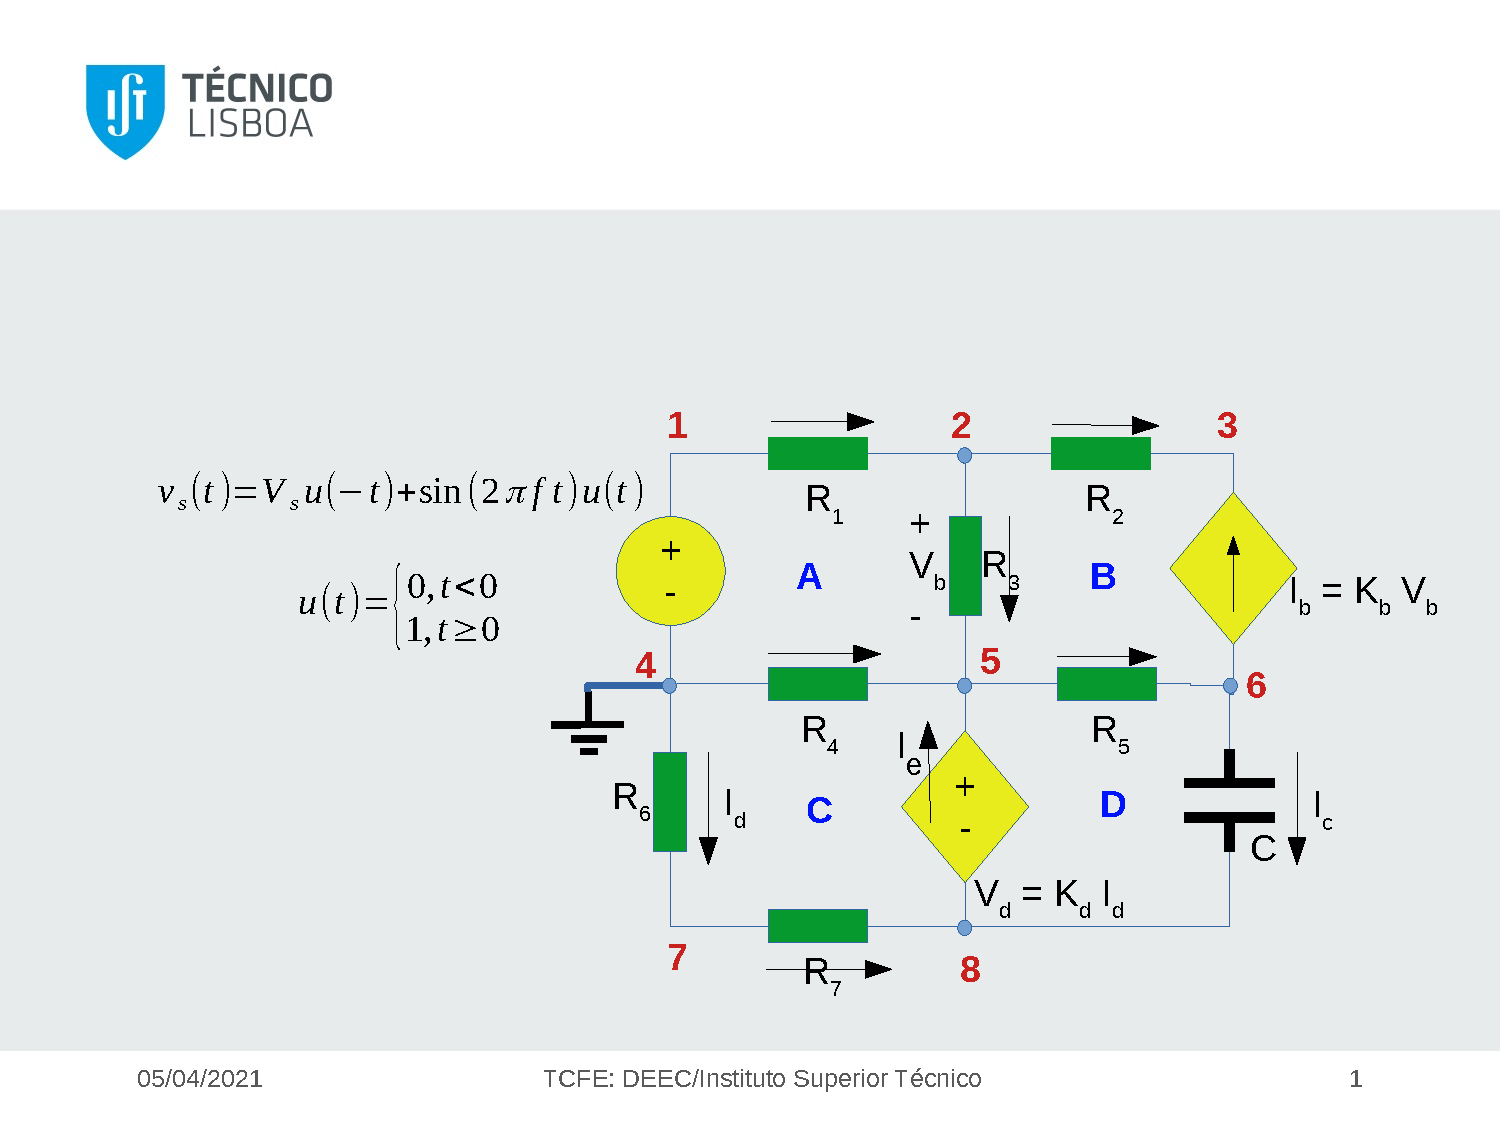
\includegraphics[width=1\linewidth]{t2.pdf}
\caption{RC circuit to be analysed}
\label{fig:t2}
\end{figure}

